%======================================================================
\chapter{ Waveguiding and Weak Measuring}
\label{Ch:wave&Weak}
%======================================================================
\textbf{This chapter is based on the following papers:}
\begin{enumerate}
    \item \textbf{Author 1}, Author 2, Author 3, and Supervisor,\\
``Weak Measuring and Waveguiding", \textit{Physical Review Re-reseach} \textbf{1}, 0326 (2026). \\ DOI: \href{https://doi.org/10.1103/PhysRevResearch.3.033226}{https://doi.org/}  
\end{enumerate}

Motivation to the chapter 

%======================================================================
\section{Wave guiding}
\label{sec:wave}
%=====================================================================
Light gets guided in a waveguide. Look at our diagram \ref{fig:Knots}.

\begin{figure}[H]
    \centering
    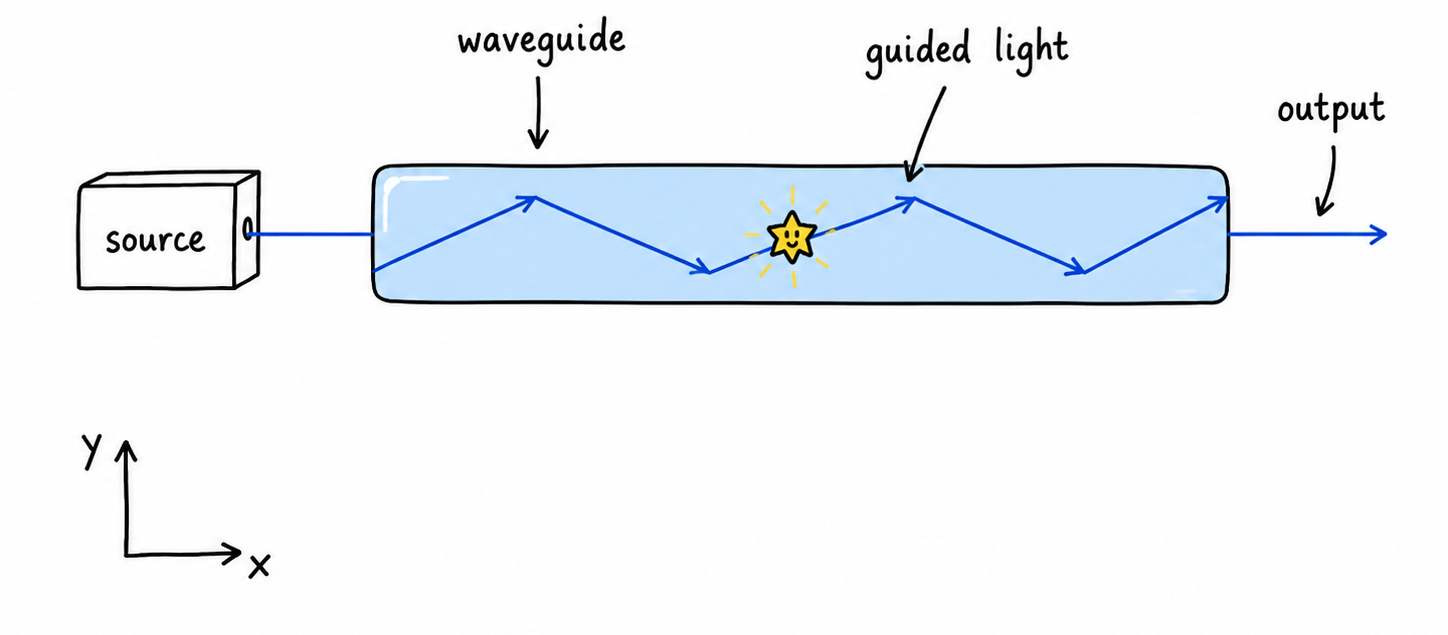
\includegraphics[width=\textwidth]{figures/C3/fig-waveguide.png}
    \caption{\textbf{Wave and their guidance.} The photon gets trapped and guided towards somewhere.}
    \label{fig:Knots}
\end{figure}


%======================================================================
\section{Weak Measuring}
\label{sec:WeakMeasuring}
%=====================================================

If you barely perturbe the system, it stays almost the same! Figure \ref{fig:weak} shows how not to do a weak measurment


\begin{figure}[H]
    \centering
    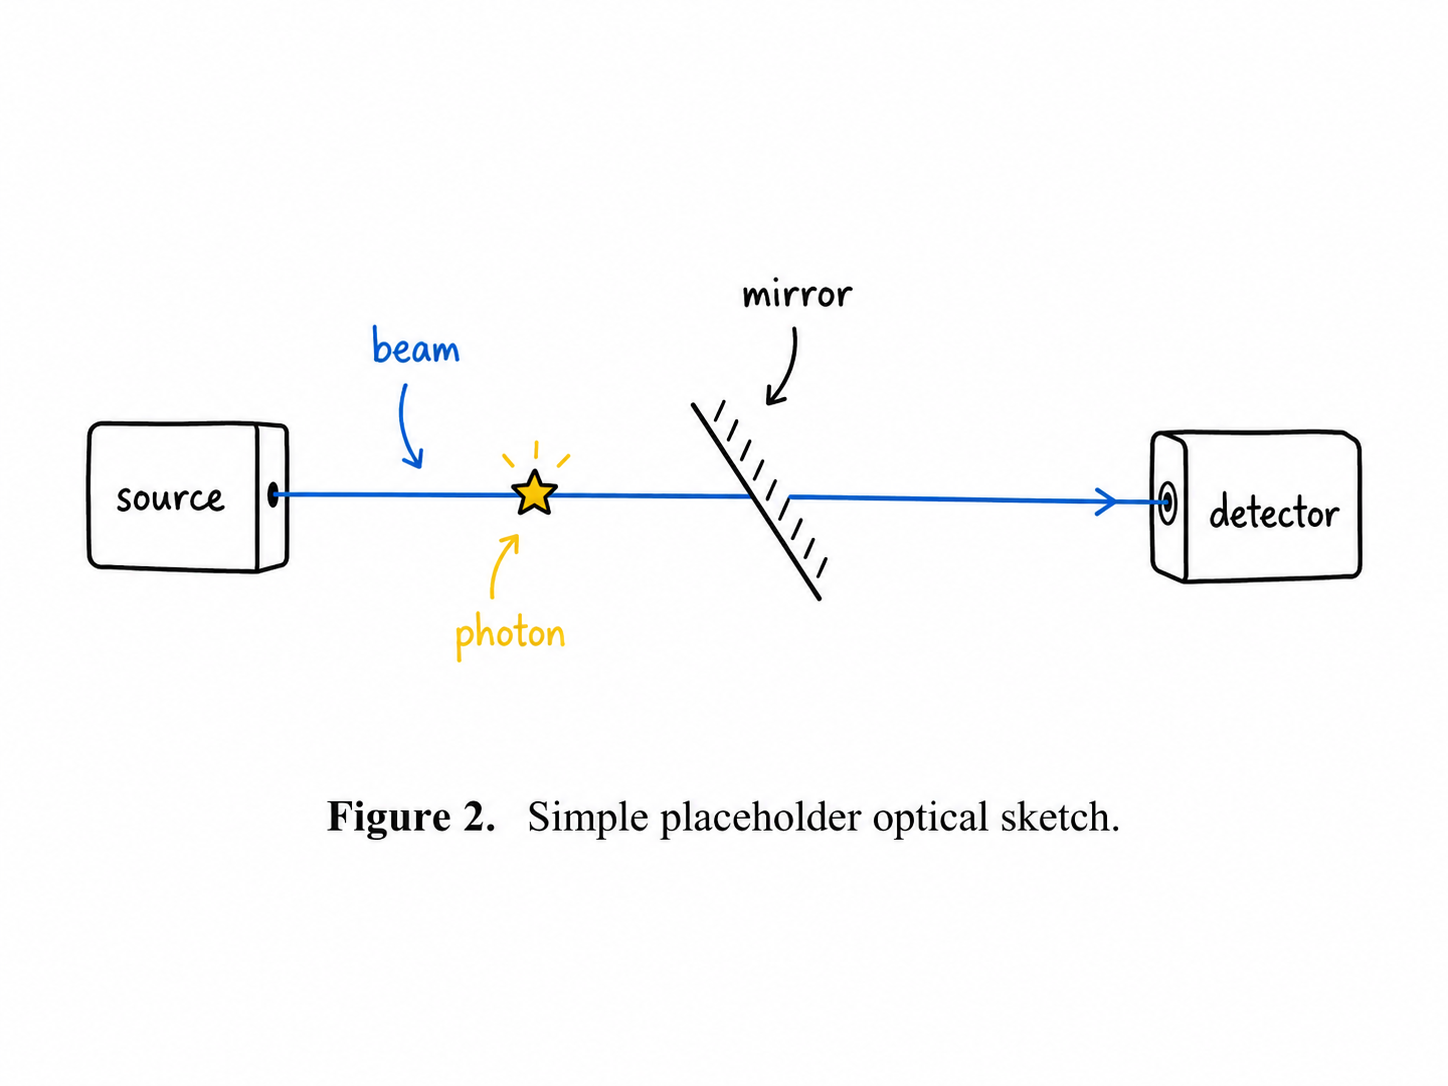
\includegraphics[width=\textwidth]{figures/C3/fig-weakMeasurment.png}
    \caption{\textbf{Example of a bad weak measurement. a.} The photon sometimes reflects or goes through. Although, I forgot to measure it. }
    \label{fig:weak}
\end{figure}


 \Publication{\textbf{Publication: } Weak and Measure
}{PDF/DummyArticle.pdf} 



